All periodic first-principles calculations performed in this study were carried out using the plane-wave density functional theory (DFT) as implemented in the Vienna Ab-initio Simulation Package (VASP) code.\cite{Kresse1996EfficiencySet},\cite{Kresse1999FromMethod} The interaction between ionic cores and valence electrons was described using the projector-augmented-wave (PAW) potentials provided with VASP. 

\begin{figure*}
  \centering
  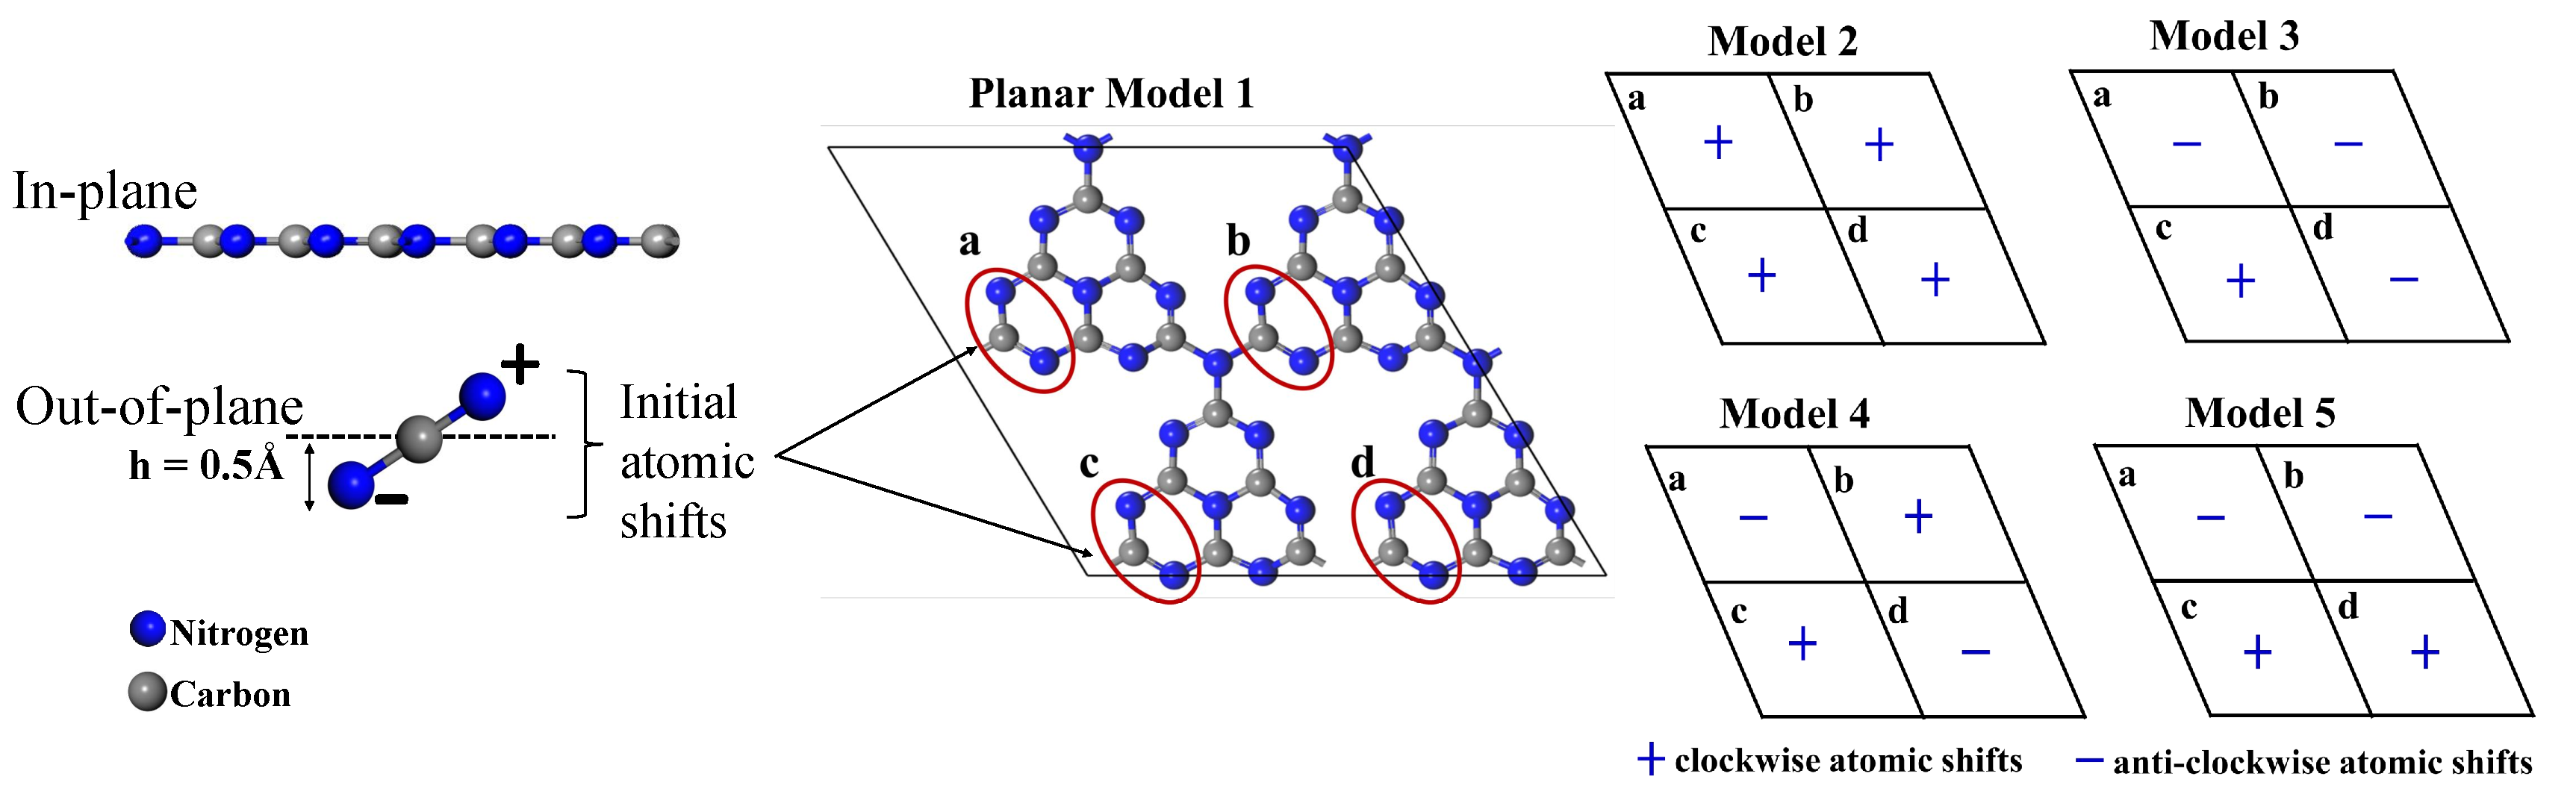
\includegraphics[width=6.5in]{Figures/Fig1.pdf}
 \caption{Exploration of low-energy g-C$_3$N$_4$ buckling patterns initiated by atomic shifts/distortions of the planar monolayer.} 
  \label{fig:Fig1} 
\end{figure*}

Exchange-correlation energies were treated within the generalized gradient approximation (GGA) using the Perdew-Burke-Ernzerhof (PBE) functional. To properly account for weak interlayer interactions in the bulk models, van der Waals corrections were included using the DFT-D3 scheme\cite{Grimme2010AH-Pu} with Becke-Johnson damping. The PBE functional without dispersion corrections as well as the r$^2$SCAN meta-GGA and HSE06 screened hybrid functionals were used for specific comparisons, as noted in the results presented below. These functionals were applied at the geometries that minimize the PBE-D3(BJ) energy. To assess the robustness of the predicted structure, one representative bulk structure was also fully optimized using different functionals (see Table S3 and Fig. S3). The plane wave energy cutoff was set as 500 eV, while the self-consistency energy convergence criterion was set to 10$^{-6}$ eV. 
All structures were based on layers comprised of $2 \times 2$ supercells of the heptazine monomeric unit and an accompanying pore. The Brillouin zone was sampled using $\Gamma$-centered k-point meshes, specifically a $3 \times 3 \times 1$ grid for 2D structures (incorporating a nominally 20~\AA\ gap between layers) and a $3 \times 3 \times 7$ grid for the 3D bulk systems. These grid point meshes were selected based on convergence tests that confirmed they are well-converged with respect to total energy (see Fig. S1). 

To systematically search for lower-energy configurations, we introduced out-of-plane shifts of 0.5~\AA\ for different atoms within heptazine to break the planar symmetry as depicted in Fig.\ \ref{fig:Fig1}. The monolayer was partitioned into four symmetry-related regions labelled a, b, c, and d. Each label corresponds to two pyridinic nitrogen atoms (N$_2$C sites), which are two-coordinated nitrogen atoms bonded to two carbon atoms within each heptazine unit. These N$_2$C atoms serve as the primary sites where out-of-plane perturbations were applied to initiate buckling. Model 1 represents the planar reference structure without any atomic perturbation, whereas Models 2 to 5 incorporate systematic clockwise ($+$) and anti-clockwise ($-$) out-of-plane atomic shifts. 

To determine the stability of P and Ni dopants in the 2D/3D g-C$_3$N$_4$ structures, we carried out spin-polarized DFT calculations.  The energy required to create a substitutional defect ($E_{\text{form}}^{\text{sub}}$) and an interstitial defect ($E_{\text{form}}^{\text{int}}$) were calculated using the following formation energy equations:
\begin{equation}
E_{\text{form}}^{\text{sub}} = E_{\text{doped}} - E_{\text{undoped}} - \mu_{\mathrm{dopant}} + \mu_{\mathrm{C/N}}
\label{eq:formation_energy_sub}
\end{equation}
\begin{equation}
E_{\text{form}}^{\text{int}} = E_{\text{doped}} - E_{\text{undoped}} - \mu_{\mathrm{dopant}}
\label{eq:formation_energy_int}
\end{equation}
where $E_{\text{doped}}$ and $E_{\text{undoped}}$ are the total energies of the doped and pristine supercells, $\mu_{\mathrm{dopant}}$ is the chemical potential of the added dopant atom, while $\mu_{\mathrm{C/N}}$ corresponds to the chemical potential of the atom that occupied the substitution site prior to doping (either C or N).
The chemical potential terms were taken as the per atom energy from the relevant pure phase: black phosphorous for P, metallic nickel for Ni, graphite for C and molecular dinitrogen (isolated in a large periodic box) for N.  Care was taken to converge the k-point grids for these pure phase calculations (Fig.~S7) to ensure that the corresponding uncertainties in Eqs.\ (\ref{eq:formation_energy_sub}) and (\ref{eq:formation_energy_int}) due to sampling were significantly smaller than the values quoted in this work.
A single dopant atom was used in each $2 \times 2$ supercell for the single layer stuctures and one dopant atom in the two layer supercell for the bulk structures.

The interlayer binding energy was calculated using the expression:\cite{Bian2022StrongMaterials,Jung2018APrinciples}
\begin{equation}
E_b = \frac{2E_{\rm single-layer} - E_{\rm bulk}}{2A}
\label{eq:binding}
\end{equation}
where \(A\) is the basal-plane area of the bulk unit cell, \(E_{\rm single-layer}\) is the total energy of the optimized monolayer, and \(E_{\rm bulk}\) is the total energy of the corresponding two-layer bulk supercell.

A limited investigation of molecular heptazine dimers was conducted using the Gaussian 16 code.\cite{Frisch2016GaussianC.01}  
Two heptazine molecules (C$_6$N$_7$H$_3$) were brought together edge to edge in a constrained relaxation, controlling the N-N distance of one intermolecular pair and maintaining the planes of the two molecules at right angles to isolate the N-N lone pair interaction. The MP2/def2-SVP level of theory was used for dimer calculations.
Moreover, limited Reverse Monte Carlo (RMC) simulations were performed on X-ray total scattering data from synthesised samples of g-C$_3$N$_4$.\cite{Adnan2026atomicallycoordinatednonmetal}  These simulations were performed with the RMCProfile code.\cite{Tucker2007RMCProfile:Materials,Liu2025HarnessingCapacitors,Wang2025RegulatedFixation}
Starting from a 10000 atom supercell of planar bulk g-C$_3$N$_4$, the RMC iteratively perturbs the positions of these atoms until the calculated scattering pattern matches the experimentally measured data.